\documentclass{resume}
\begin{document}
\fontfamily{ppl}\selectfont
\noindent
\begin{tabularx}{\linewidth}{@{}m{0.75\textwidth} m{0\textwidth}@{}}
{
    \large {Martin Augusto Rosales Figueroa} \newline
    \small{
    % \begin{align}
    %     Your Tagline\newline
    % \end{align}
    Lima, Peru \newline
    martinrosalesfg@gmail.com \newline
     +51 935 349 835 
     
    % https://goo.gl/maps/Z2fbMfH7AwJycmA66
    % Gudivada, Andhra Pradesh, India 
        \clink{
            % \textbf{·}
            % \href{https://codelock54.github.io/}{Portfolio} 
            %\href{martinrosalesfg@gmail.com}{Mail ID} \textbf{·}
            %\href{}{935349835}
            \textbf{·}
             \href{https://github.com/codelock54/}{GitHub}
             \textbf{·}
             \href{https://www.linkedin.com/in/martin-rosales-3bb7b8280/}{LinkedIn}
             % \textbf{·} 
             % \href{https://link-to-your-video-resume (if exists)}{Video Resume}
        } \newline
    }
}
& 
{
    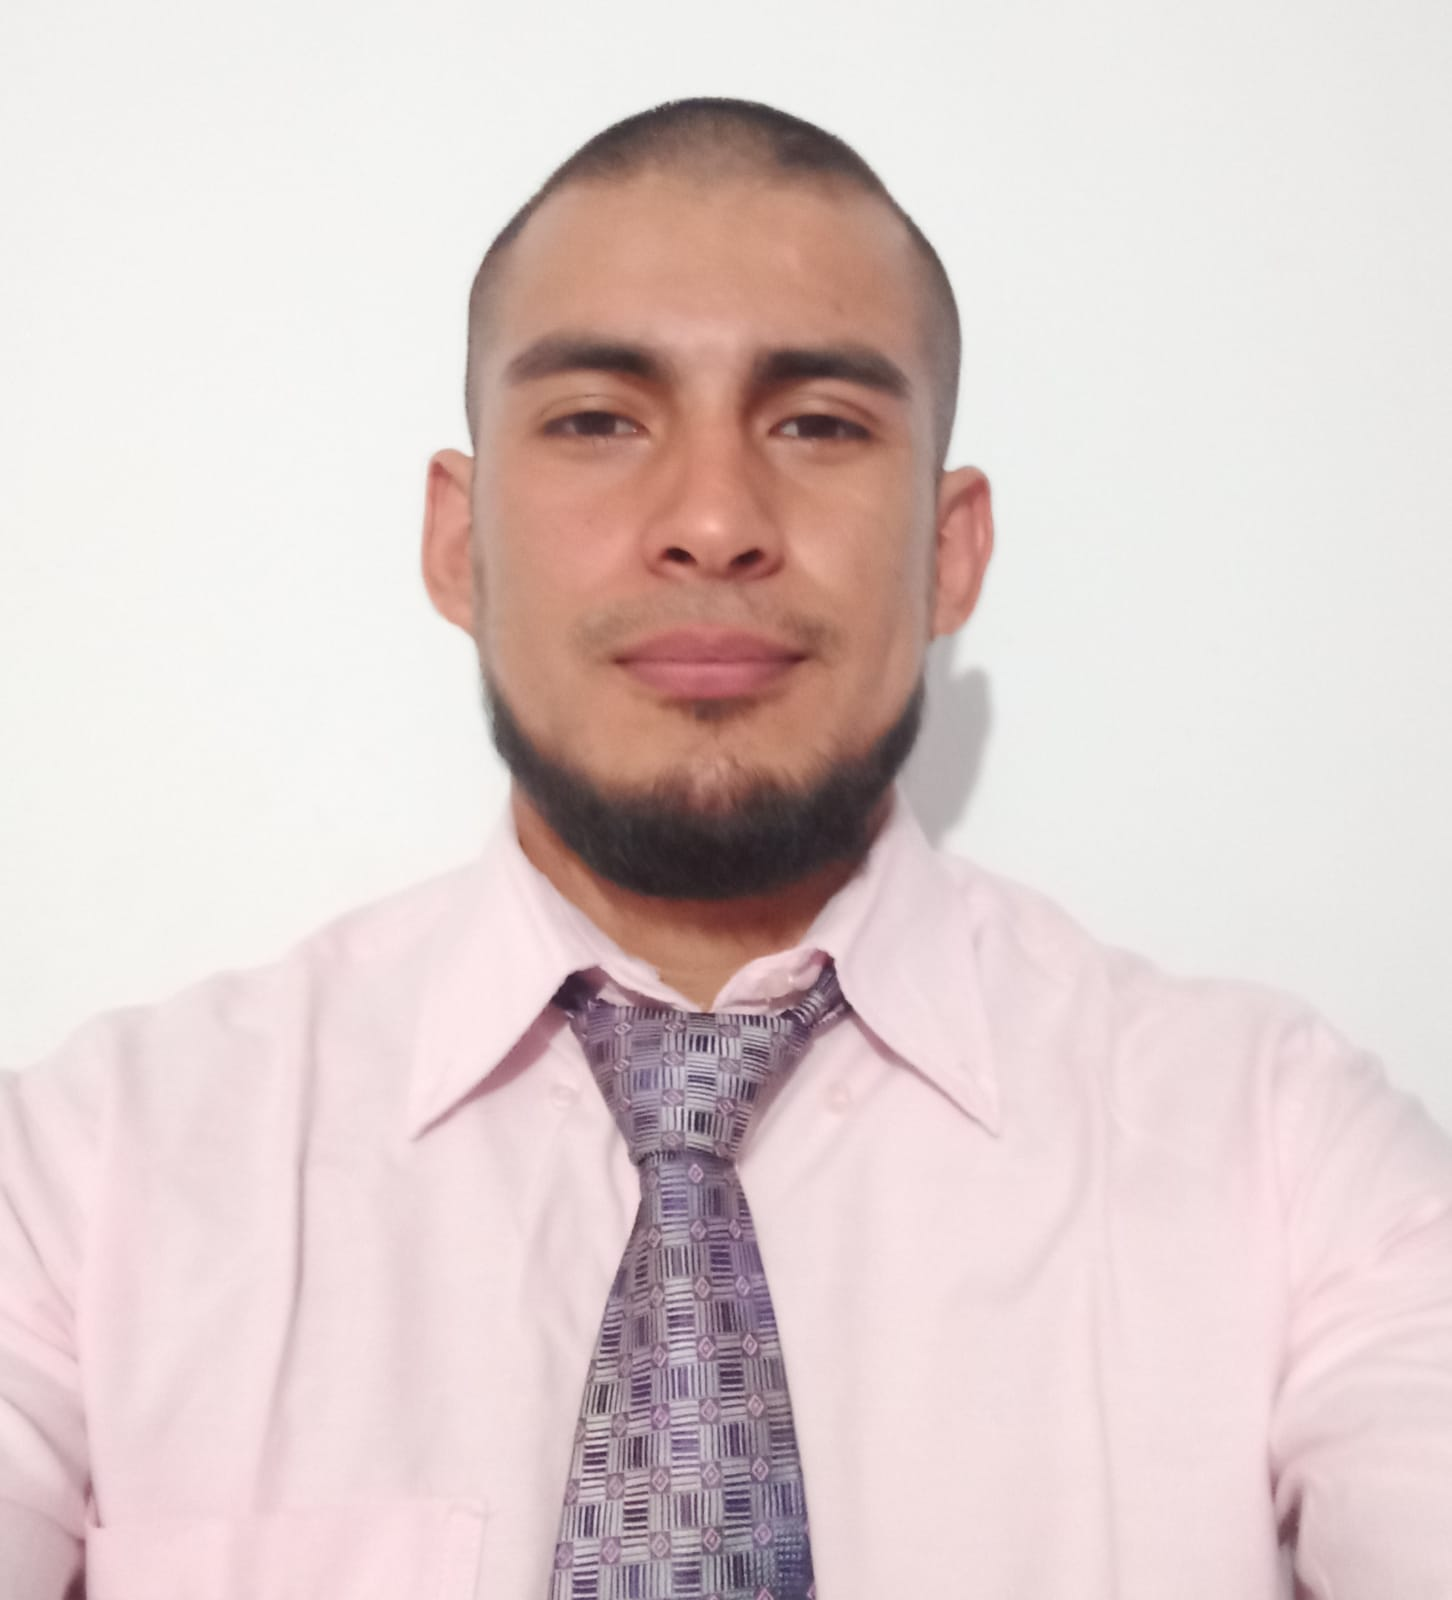
\includegraphics[width=4cm]{Photo2.jpeg}
}
\end{tabularx}
\csection{Perfil}{\small
    \begin{itemize}
        \item \footnotesize 

Soy un motivado y dedicado data scientist con sólidos conocimientos y pasión por participar en proyectos y resolver problemas
complejos. Conocimiento en estadística, matematicas, machine learning y visualización de datos. Manejo de lenguaje Python, C
++, Matlab y SQL con experiencia en data engineer, preprocessing, desarrollo y despliegue de modelos. Soy de aprendizaje
rapido, adaptable y con ganas de seguir aprendiendo y profundizando mas mis conocimientos para aplicarlos en escenarios del
mundo real.
    \end{itemize}
}
\csection{EDUCACION}{\small
    \begin{itemize}
        % item 1 %
        \item \textbf{Universidad\hspace{29em}(2019-2025)}\newline{ESAN (Computer Science Engineering)}%\newline{Marks/CGPA: your marks/cgpa}
        \item \textbf{Cursos}\newline\textbf{- }{Machine Learning by Standford University(Coursera) }\href{https://github.com/codelock54/Stanford-University-ML-Course}{Link}\hspace{4em}Abril 2022 - Julio 2022
        \item \textbf{Libros}\newline\textbf{- }{Hands-on Machine Learning with Scikit-Learn, Keras, and TensorFlow}
        % \item \textbf{Intermediate or Diploma\hspace{25.5em}(20xx - 20xx)}\newline{Your intermediate or diploma college.}\newline{Marks/CGPA: your marks/cgpa}{}
        
        % \item\textbf{High School\hspace{31.65em}(20xx - 20xx)}\newline{Your School.}\newline{Marks/CGPA: your marks/cgpa}{}
        
    \end{itemize}
}
 
\csection{SKILLS}{\small
    \begin{itemize}
        \item \textbf{Lenguajes de programacion} \newline
        {\footnotesize Python Intermedio \newline 
        C++ intermedio  \newline
        Matlab basico}{}{}
        
        \item \textbf{Libraries/Frameworks} \newline
        {\footnotesize TensorFlow, Keras, Sklearn, Pandas, Numpy,  matplotlib}{}{}
        
        \item \textbf{Cloud} \newline
        {\footnotesize AWS (IAM, EC2, Sagemaker, Lambda, S3, Step Functions, Glue, EBS, ECR, RDS, Athena, Kinesis, etc)}{}{}
        
        \item \textbf{Databases} \newline
        {\footnotesize MYSQL, SQL Sever, MongoDB}{}{}

        \item \textbf{OS} \newline
        \textbf {Linux:} \newline 
       {\footnotesize  Ubuntu server, Ubuntu desktop, Kali Linux} \newline 
        \textbf{Windows:}\newline 
        {\footnotesize Windows Server, Windows 10}

        \item \textbf{Virtual Machine} \newline
        {\footnotesize Virtual box, Qemu} 
        
         \item \textbf{Office} \newline
        {\footnotesize Excel intermedio \newline
        Power BI Intermedio \newline
        Word Intermedio \newline
        PowerPoint Intermedio \newline}{}{}
  
        
        \item \textbf{Idiomas} \newline
        {\footnotesize English: B2    \newline
        Spanish: C2 \newline
        Japanese: A2 \newline
        Portuguese: A2 \newline}

          \item \textbf{Otros Skills} \newline
        {\footnotesize Data Science, Data Analysis, Machine Learning, Data Engineer\newline
         Git/GitHub, Docker }
         
    \end{itemize}
       }

%\csection{PROJECTS}{\small
 %   \begin{itemize}
       
 %   \end{itemize}
%}
    
\csection{PROYECTOS/ OPEN SOURCE}{\small
    \begin{itemize}
       \item \textbf{\href{https://github.com/codelock54/Airbnb_model}{Airbnb Price Prediction}}
       
       \item \textbf{\href{https://github.com/codelock54/Book_Price}{Book Price Prediction}}
       
       \item \textbf{\href{https://github.com/codelock54/Happiness-Rank-2015}{Happiness Score 2015 }}
       
       \item \textbf{\href{https://github.com/codelock54/Airbnb_model}{Brain Tumor Classification}}
       
       \item \textbf{\href{https://github.com/codelock54/Juego-Ahorcado}{Hangman Game in c++}}
       
       \item \textbf{\href{https://github.com/codelock54/Brain-tumor-Classification}{Drug Classification}}
       
    \end{itemize}
}
    

%\csection{Significant Roles}{\small
 %   \begin{itemize}
       % \item \textbf{Name of your role \hspace{17.5em}Month Year – Month Year (Duration)}\newline{Location}{}{}{}
        
        % \item \textbf{Peer Mentor \hspace{25em}MAY '21 – MAY '22 (12 M)}\newline{K L University }{}{}{}
        
        % \item \textbf{Student Member of CSE  IRP CELL \hspace{15em}OCT '20 – MAY '21 (8 M)}\newline{K L University}{}{}{}
 %   \end{itemize}
%}
    
\csection{EXPERIENCIA}{\small
    \begin{itemize}
        \item \textbf{Cienporciento SAC \hspace{22em}Jan 2022 – july 2023 }\newline{Programador: desarrollo de programas en Python, administracion de servidores Linux, consultas SQL, configurarion de redes, trabajo con la nube de AWS(S3, EC2, IAM, Lambda, RDS, VPC, subnets, Security Groups, Developer tools, etc)}{}{}{}
        
    \end{itemize}
}
    
\csection{CERTIFICACIONES}{\small
    \begin{itemize}
        \item \textbf{AWS Cloud Practitioner}  {\footnotesize \hspace{1em}\href{https://www.credly.com/badges/fac9cee0-d332-46b0-bf33-0e9d38b2c658/public\_urlw}{Link}}
        {\hspace{20em}Overall Score: 750}{}{}

         \item \textbf{SQL (Intermediate) Certificate}  {\footnotesize \hspace{1em}\href{https://www.hackerrank.com/certificates/97d7915a72b7}{Link}}
        {}{}

         \item \textbf{Python (Intermediate) Certificate}  {\footnotesize \hspace{1em}\href{https://www.sololearn.com/certificates/CT-ZFFTJ6NZ}{Link}}
        {}{}

        \item \textbf{Machine Learning Certificate}  {\footnotesize \hspace{1em}\href{https://www.sololearn.com/certificates/CT-ZMQ36G73}{Link}}
        {}{}
    \end{itemize}
    
  
}
        
\csection{Referencias}{\small
    \begin{itemize}
        \item \textbf{Ing. Cesar Peralta \hspace{27em}{+51 949 699 944}}\newline{\footnotesize Cienporciento SAC. }{}
    \end{itemize}
    % \begin{itemize}
    %     \item \textbf{Anne Venkata Praveen Krishna Sir}\newline{\footnotesize Placements Incharge, CSE, KLU.\hspace{33.25em}\href{tel:9949395595}{Contact}}{}
    % \end{itemize}
}

% \csection{Declaration}{\small
%     \begin{itemize}
%         \item \footnotesize I hereby declare that the above mentioned information is correct up to my knowledge and I bear the responsibility for the correctness of the above mentioned.
%     \end{itemize}
% }

\end{document}
